% ===== CHAPTER 10 =====
\chapter{电子自旋和自旋-统计定理}
\label{chap:10}
\section{电子自旋}
\label{sec:10.1 Electron Spin}

    所有化学家都熟悉钠原子在火焰中呈现的黄色。事实上,钠原子光谱中最强的黄色线(D线)是两条间隔很近的线。钠的D谱线由激发态$1s^22s^22p^63p$到基态的跃迁产生。\ce{Na} 光谱中这条线和其他线的双线性质表明,价电子可用的预期状态数增加了一倍。

    为了解释原子光谱的这种微观结构,Uhlenbeck 和 Goudsmit 于 1925 年提出,除了电子围绕原子核运动所产生的轨道角动量之外,电子还具有一种\textit{内禀}(内在)角动量。如果我们把电子想象成一个围绕其直径之一旋转的电荷球,我们就能明白这种内禀角动量是如何产生的。因此,我们得到了术语\textbf{自旋角动量}(spin angular momentum),或更简单地,\textbf{自旋}(spin)。然而,电子 “自旋”并不是一种经典效应,电子绕轴旋转的图景并不符合物理现实。内禀角动量是真实存在的,但没有一个容易又直观的模型能够正确解释它的起源。我们不能指望根据宏观世界的经验来理解微观粒子。除了电子,其他基本粒子也有自旋角动量。

    1928 年,狄拉克提出了电子相对论量子力学,在他的研究中,电子自旋自然而然地产生了。

    在我们所局限的非相对论量子力学中,电子自旋必须作为附加假设引入。我们已经了解到,在量子力学中,每种物理属性都有其对应的线性厄米算符。对于轨道角动量等性质,我们可以用相应的算符代替 $p_x$、$p_y$和$p_z$,从经典表达式中构造出量子力学算符。微观粒子固有的自旋角动量在经典力学中没有类似的表达式,因此我们不能用这种方法来构造自旋的算符。为了我们的目的,我们将只使用符号来表示自旋算符,而不给出它们的明确形式。

    与轨道角动量算符$\hat{L}^2, \hat{L}_x, \hat{L}_y, \hat{L}_z$类似,自旋算符也有对应的形式$\hat{S}^2, \hat{S}_x, \hat{S}_y, \hat{S}_z$,假设它们是线性厄米算符。$\hat{S}^2$ 是粒子总自旋角动量大小平方的算符。$\hat{S}_z$ 是自旋角动量在 $z$ 方向上的分量算符。我们有
    \begin{equation}
        \hat{S}^2 = \hat{S}_x^2 + \hat{S}_y^2 + \hat{S}_z^2.
        \label{eq:10.1}
    \end{equation}
    假设自旋角动量算符遵循轨道角动量算符相同的对易关系。与$\left[\hat{L}_x, \hat{L}_y\right] = \mathrm{i} \hbar \hat{L}_z$,$\left[\hat{L}_y, \hat{L}_z\right] = \mathrm{i} \hbar \hat{L}_x$,$\left[\hat{L}_z, \hat{L}_x\right] = \mathrm{i} \hbar \hat{L}_y$[式(\ref{eq:5.46})和(\ref{eq:5.48})],我们有
    \begin{equation}
        \left[\hat{S}_x, \hat{S}_y\right] = \mathrm{i} \hbar \hat{S}_z, \quad
        \left[\hat{S}_y, \hat{S}_z\right] = \mathrm{i} \hbar \hat{S}_x, \quad
        \left[\hat{S}_z, \hat{S}_x\right] = \mathrm{i} \hbar \hat{S}_y.
        \label{eq:10.2}
    \end{equation}
    根据(\ref{eq:10.1})和(\ref{eq:10.2}),通过求得(\ref{eq:5.49})和(\ref{eq:5.50})时所用的算符代数,可以得出
    \begin{equation}
        \left[\hat{S}^2, \hat{S}_x\right] = \left[\hat{S}^2, \hat{S}_y\right] = \left[\hat{S}^2, \hat{S}_z\right] = 0
        \label{eq:10.3}
    \end{equation}
    由于公式 (\ref{eq:10.1}) 和 (\ref{eq:10.2}) 是公式 (\ref{eq:5.107}) 和 (\ref{eq:5.108}) 的形式,根据第 \ref{sec:5.4 The Ladder-Operator Method for Angular Momentum} 节的工作(只取决于对易关系,而不取决于算符的具体形式),可以得出 $\hat{S}^2$ 的本征值为[式(\ref{eq:5.142})]
    \begin{equation}
        \boxed{
            s\left(s+1\right)\hbar^2, \quad s = 0, \frac{1}{2}, 1, \frac{3}{2}, \ldots
        }
        \label{eq:10.4}
    \end{equation}
    以及$\hat{S}_z$ 的本征值为[式(\ref{eq:5.141})]
    \begin{equation}
        \boxed{
            m_s\hbar, \quad m_s = -s, -s+1, \ldots, s-1, s
        }
        \label{eq:10.5}
    \end{equation}

    量子数$s$称为粒子的\textbf{自旋量子数}(spin quantum number)。尽管第 \ref{sec:5.4 The Ladder-Operator Method for Angular Momentum} 节中并没有限制电子的 $s$ 值只能是单一的,但实验表明,所有电子的 $s$ 值都是单一的,即$s = \frac{1}{2}$。质子和中子同样有$s = \frac{1}{2}$。离子有$s = 0$。光子则有$s=1$。然而,公式 (\ref{eq:10.5}) 对光子并不成立。光子在真空中以 $c$ 的速度传播。由于其相对论性质,光子可以有以下两种情况:$m_s = +1$ 或 $m_s = -1$,但不具有$m_s = 0$(见\textit{Merzbacher}, Chapter 22)。这两个 $m_s$ 值分别对应左旋圆偏振光和右旋圆偏振光。

    有了$s = \frac{1}{2}$,电子总自旋角动量的值由(\ref{eq:10.4})的平方根给出:
    \begin{equation}
        \left[\frac{1}{2}\left(\frac{3}{2}\right)\hbar^2\right]^{1/2}=\frac{1}{2}\sqrt{3}\hbar
        \label{eq:10.6}
    \end{equation}
    对于$s = \frac{1}{2}$,式(\ref{eq:10.5})给出了电子$\hat{S}_z$的可能本征值为$+ \frac{1}{2}\hbar$和$-\frac{1}{2}\hbar$。因对应于这些$\hat{S}_z$本征值的电子自旋本征函数由$\alpha$和$\beta$给出:
    \begin{equation}
        \boxed{
            \hat{S}_z \alpha = + \frac{1}{2}\hbar \alpha
        }
        \label{eq:10.7}
    \end{equation}
    \begin{equation}
        \boxed{
            \hat{S}_z \beta = - \frac{1}{2}\hbar \beta
        }
        \label{eq:10.8}
    \end{equation}
    由于$\hat{S}_z$和$\hat{S}^2$可对易,我们可以将$\hat{S}_z$的本征函数变为$\hat{S}^2$的本征函数,有了$s = \frac{1}{2}$和(\ref{eq:10.4})给出的本征值,我们有
    \begin{equation}
        \hat{S}^2 \alpha = \frac{3}{4}\hbar^2 \alpha, \quad
        \hat{S}^2 \beta = \frac{3}{4}\hbar^2 \beta
        \label{eq:10.9}
    \end{equation}
    $\hat{S}_z$和$\hat{S}_x$、$\hat{S}_y$不可对易,所以$\alpha$和$\beta$不是$\hat{S}_x$和$\hat{S}_y$的本征函数。术语\textit{自旋向上}(spin up)和\textit{自旋向下}(spin down)分别指的是$m_s = +\frac{1}{2}$和$m_s = -\frac{1}{2}$。见图10.1。稍后我们将证明,量子数 $m_s$ 的两种可能性会使碱金属光谱中的谱线条数加倍。
    \begin{figure}[ht]
        \centering
        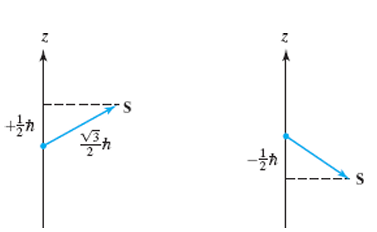
\includegraphics[width=0.4\textwidth]{Figures/10.1.png}
        \caption{
            \centering
            \parbox{\linewidth}{
                \centering 
                电子自旋矢量相对于 $z$ 轴的可能方向。在每种\\
                情况下,$\mathbf{S}$ 都位于以 $z$ 轴为轴的圆锥表面上。
            }
        }
        \label{fig:10.1}
    \end{figure}

    我们之前讨论过的波函数是粒子空间坐标的函数:$\psi = \psi\left(x,y,z\right)$。我们可能想问:自旋本征函数$\alpha$和$\beta$的变量是什么呢?有时,人们在谈论自旋坐标 $\omega$ 时,并没有明确说明这个坐标是什么。通常情况下,人们把自旋量子数 $m_s$ 作为自旋特征函数所依赖的变量。与空间波函数相比,这种程序很不寻常;但因为我们只有两种可能的电子自旋特征函数和本征值,所以这是一种方便的选择。我们有
    \begin{equation}
        \alpha = \alpha\left(m_s\right), \quad
        \beta = \beta\left(m_s\right)
        \label{eq:10.10}
    \end{equation}

    像往常一样,我们希望对本征函数进行归一化处理。单粒子空间波函数的三个变量范围在$-\infty$到$+\infty$之间连续变化,则归一化条件意味着
    \begin{equation*}
        \int_{-\infty}^{\infty} \int_{-\infty}^{\infty} \int_{-\infty}^{\infty} \left|\psi\left(x, y, z\right)\right|^2\: \mathrm{d}x\: \mathrm{d}y\: \mathrm{d}z = 1
    \end{equation*}
    电子自旋本征函数的变量 $m_s$ 只有 $+\frac{1}{2}$ 和 $-\frac{1}{2}$ 两个离散值。因此,对单粒子自旋本征函数的归一化意味着
    \begin{equation}
        \sum_{m_{s}=-1/2}^{1/2} \left|\alpha \left(m_{s}\right)\right|^{2} = 1, \quad \sum_{m_{s}=-1/2}^{1/2} \left|\beta \left(m_{s}\right)\right|^{2} = 1
        \label{eq:10.11}
    \end{equation}
    因为本征函数$\alpha$和$\beta$对应于厄米算符$\hat{S}_z$的不同本征值,所以它们是正交的:
    \begin{equation}
        \sum_{m_{s}=-1/2}^{1/2} \alpha^ * \left(m_{s}\right) \beta \left(m_{s}\right) = 0
        \label{eq:10.12}
    \end{equation}
    令$\alpha\left(m_s\right) = \delta_{m_s, 1/2}$,$\beta\left(m_s\right) = \delta_{m_s, -1/2}$,其中$\delta_{jk}$是Kronecker $\delta$函数,我们就满足了(\ref{eq:10.11})和(\ref{eq:10.12})。

    当我们考虑电子的完全波函数(包括空间和自旋变量)时,我们将根据以下公式对其进行归一化处理
    \begin{equation}
        \boxed{
            \sum_{m_s=-1/2}^{1/2} \int_{-\infty}^{\infty} \int_{-\infty}^{\infty} \int_{-\infty}^{\infty} \left|\psi\left(x, y, z, m_s\right)\right|^2 \:\mathrm{d}x \:\mathrm{d}y \:\mathrm{d}z = 1
        }
        \label{eq:10.13}
    \end{equation}
    符号
    \begin{equation*}
        \int \left|\psi\left(x, y, z, m_s\right)\right|^2 \:\mathrm{d}\tau
    \end{equation*}
    表示对自旋变量求和,对空间变量全范围积分,如 (\ref{eq:10.13}) 所示。符号 $\int \:\mathrm{d}v$ 表示对系统空间变量全范围的积分。

    \begin{quote}
        \small
        \noindent
        电子目前被认为是一种没有子结构的点状基本粒子。高能电子-正电子碰撞实验表明,没有证据表明电子的大小不为零,并将电子半径的上限为$3 \times 10^{-19} \:\mathrm{m}$[D. Bourilkov, \textit{Phys. Rev. D}, \textbf{62}, 076005 (2020); \url{arxiv.org/abs/hep-ph/0002172}.]。质子和中子是由夸克构成的,因此不是基本粒子。质子的均方根电荷半径为$0.88 \times 10^{-15} \:\mathrm{m}$。
    \end{quote}

\section{自旋和氢原子}
\label{sec:10.2 Spin and the Hydrogen Atom}

    具体说明电子状态的波函数不仅取决于$x$、$y$和$z$坐标,还取决于电子的自旋状态。这对氢原子的波函数和能级有什么影响?

    在很好的近似条件下,电子系统的哈密顿算符不涉及自旋变量,而只是空间坐标和关于空间坐标的导数的函数。因此,我们可以将单个电子的定态波函数分离为空间和自旋部分的乘积:
    \begin{equation*}
        \psi\left(x,y,z\right)g\left(m_s\right)
    \end{equation*}
    其中的$g\left(m_s\right)$是$\alpha$或$\beta$的其中之一,取决于$m_s = +\frac{1}{2}$或$m_s = -\frac{1}{2}$。[更一般地,$g\left(m_s\right)$可以是$\alpha$和$\beta$的线性组合;$g\left(m_s\right) = c_1 \alpha + c_2\beta$。]由于哈密顿算符对自旋波函数没有作用,我们有
    \begin{equation*}
        \hat{H} \left[\psi\left(x, y, z\right) g\left(m_s\right)\right] = g\left(m_s\right) \hat{H} \psi\left(x, y, z\right) = E \left[\psi\left(x, y, z\right) g\left(m_s\right)\right]
    \end{equation*}
    我们得到了与之前未考虑自旋时相同的能量。引入自旋唯一的不同是使得可能的状态数翻倍。与状态$\psi\left(x, y, z\right)$不同,我们有两个可能的状态$\psi\left(x, y, z\right) \alpha$和$\psi\left(x, y, z\right) \beta$。当我们考虑自旋时,氢原子能级的简并度是$2n^2$而不是$n^2$。

\section{自旋-统计定理}
\label{sec:10.3 Spin-Statistics Theorem}














\section{氦原子}
\label{sec:10.4 Th Helium Atom}

\section{Pauli不相容原理}
\label{sec:10.5 The Pauli Exclusion Principle}

\section{Slater行列式}
\label{sec:10.6 Slater Determinants}

\section{微扰理论求解基态锂原子}
\label{sec:10.7 Perturbation Treatment of the Lithium Ground State}

\section{变分法求解基态锂原子}
\label{sec:10.8 Variation Treatments of the Lithium Ground State}

\section{自旋磁矩}
\label{sec:10.9 Spin Magnetic Moment}

\section{电子自旋的梯度算符}
\label{sec:10.10 Ladder Operators for Electron Spin}

\section*{总结}

\section*{习题}